\documentclass{article}
\usepackage{tikz}
\usetikzlibrary{intersections}
\usetikzlibrary{arrows.meta}
\begin{document}
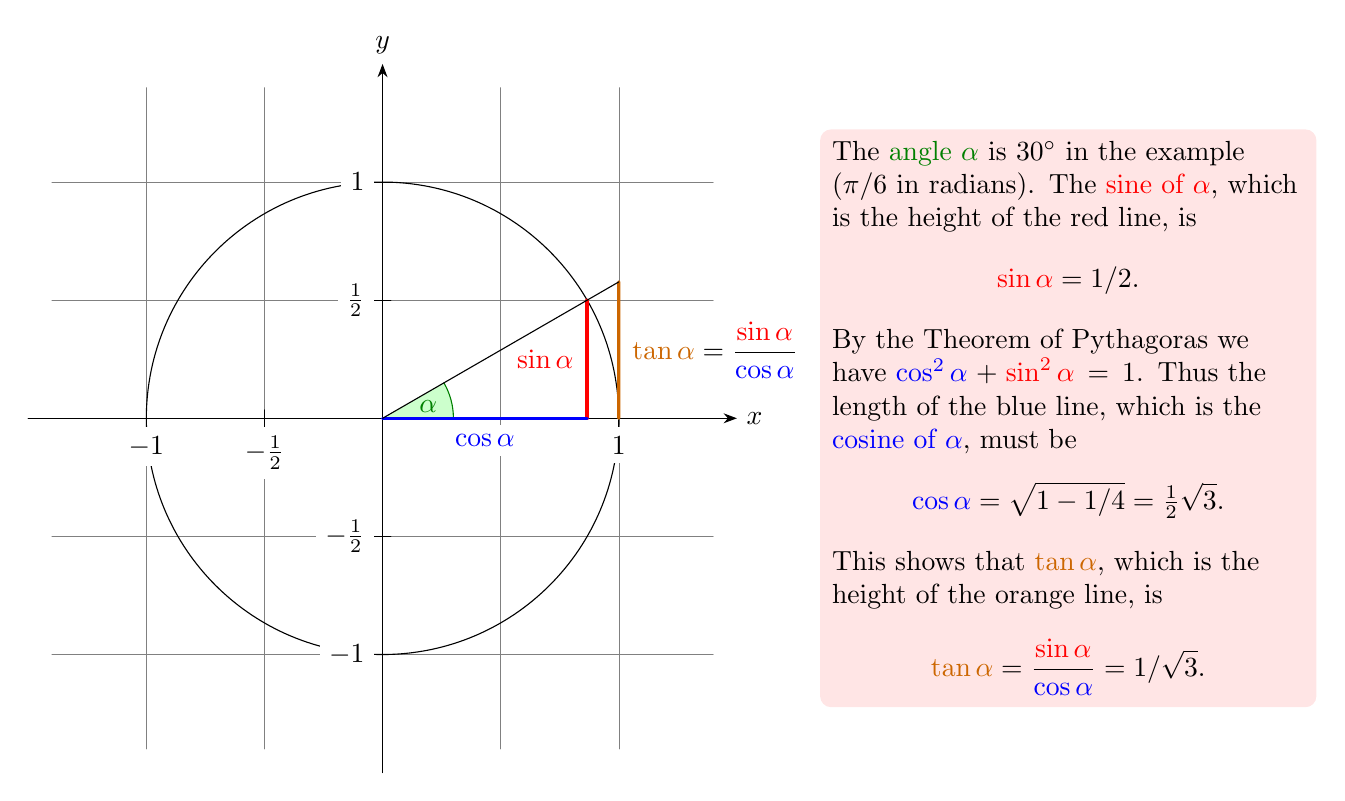
\begin{tikzpicture}[scale=3,>=Stealth,line cap=round,axes/.style=,important line/.style={very thick},information text/.style={rounded corners,fill=red!10,inner sep=1ex}]
 \colorlet{anglecolor}{green!50!black}
 \colorlet{sincolor}{red}
 \colorlet{tancolor}{orange!80!black}
 \colorlet{coscolor}{blue}
 
 \draw[help lines,step=0.5cm] (-1.4,-1.4) grid (1.4,1.4);
 \draw (0,0) circle [radius=1cm];

 \begin{scope}[axes]
 \draw[->] (-1.5,0) -- (1.5,0) node[right] {$x$} coordinate (x axis);
 \draw[->] (0,-1.5) -- (0,1.5) node[above] {$y$} coordinate (y axis);
 \foreach \x/\xtext in {-1,-0.5/-\frac12,1}
    \draw (\x cm,1pt) -- (\x cm,-1pt) node[anchor=north,fill=white] {$\xtext$};
 \foreach \y/\ytext in {-1,-0.5/-\frac12,0.5/\frac12,1}
    \draw (1pt,\y cm) -- (-1pt,\y cm) node[anchor=east,fill=white] {$\ytext$};
 \end{scope}

 \filldraw[fill=green!20!white,draw=anglecolor]
    (0,0) --
    (3mm,0mm) arc [start angle=0,end angle=30,radius=3mm];
 \draw (15:2mm) node[anglecolor] {$\alpha$};
 
 \draw[important line,sincolor] (30:1cm) -- node[left=1pt,fill=white] {$\sin\alpha$} (30:1cm |- x axis);
 \draw[important line,coscolor] (30:1cm |- x axis) -- node[below=2pt,fill=white] {$\cos\alpha$} (0,0);
 \path[name path=upwards line] (1,0) -- (1,1);
 \path[name path=sloped line] (0,0) -- (30:1.5cm);
 \draw[name intersections={of=upwards line and sloped line, by=t}]
    [important line, tancolor] (1,0) -- node[right=1pt,fill=white] {$\displaystyle\tan\alpha\color{black}=\frac{\color{red}\sin\alpha}{\color{blue}\cos\alpha}$} (t);
 \draw (0,0) -- (t);
 
 \draw[xshift=1.85cm]
    node[right,text width=6cm,information text] {
        The {\color{anglecolor}angle $\alpha$} is
        $30^\circ$ in the example ($\pi/6$ in radians).
        The {\color{sincolor}sine of $\alpha$}, which is
        the height of the red line, is
        \[
         {\color{sincolor}\sin\alpha} = 1/2.
        \]
        By the Theorem of Pythagoras we have
        ${\color{coscolor}\cos^2\alpha}+{\color{sincolor}\sin^2\alpha}=1$. Thus the length of the blue line,
        which is the {\color{coscolor}cosine of $\alpha$}, must be
        \[
         {\color{coscolor}\cos\alpha}=\sqrt{1-1/4}={\textstyle\frac12}\sqrt3.
        \]
        This shows that ${\color{tancolor}\tan\alpha}$, which is
        the height of the orange line, is
        \[
         {\color{tancolor}\tan\alpha}=\frac{\color{sincolor}\sin\alpha}{\color{coscolor}\cos\alpha}=1/\sqrt3.
        \]



    };
\end{tikzpicture}
\end{document}
